\documentclass{scrartcl}
\setkomafont{disposition}{\normalfont\bfseries}
\usepackage[utf8]{inputenc}
\usepackage{natbib}
\usepackage{graphicx}
\usepackage[a4paper,margin=1in]{geometry}
\usepackage{rotating}
\usepackage[francais]{babel}
\usepackage[T1]{fontenc}
\usepackage{xcolor}
\usepackage{hyperref}
\usepackage{amsmath}
\usepackage{listings}
\usepackage{calc}
\usepackage{xparse}
\usepackage{framed}
\usepackage{amssymb}
\usepackage{amsfonts}
\usepackage{tabularx}
\usepackage{makecell}
\usepackage{float}
\usepackage{listings}
\lstset{ 
  basicstyle=\footnotesize,
  commentstyle=\color{green},
  frame=single,
  keywordstyle=\color{blue},
  language=Java,
  rulecolor=\color{black},
  stringstyle=\color{red},
  tabsize=2,
  title=\lstname
}
\usepackage[nottoc]{tocbibind}

% Macro structuration des besoins. Trois arguments (dans l'ordre) :
% - Titre;
% - Priorité (Faible, Moyenne ou Forte);
% - Description;
\newcommand{\requirement}[3] {
\vbox{
    \begin{framed}
        {\centering \textbf{\underline{#1}}\\[0.25 cm]\par}
        \begin{itemize}
            \item \textbf{Priorité} : #2
            \item \textbf{Description} : #3
        \end{itemize}
    \end{framed}
}
}
% Macro structuration Procédure de tests des besoins.
\newcommand{\testRequirement}[1] {
    \vspace{-10px}
    $\rightarrow$ \textbf{Test} : #1
}

\newcommand{\project}{$\mathbf{\Pi}$}
\newcommand{\classUniverse}{$\mathbf{U}$}
\newcommand{\category}{$\mathbf{C}$}
\newcommand{\class}{$c$}

\newcommand{\categoryUniverse}{$\mathbf{P}$}
\newcommand{\dependantClasses}{$\mathbf{DaC}$}
\newcommand{\dependedClasses}{$\mathbf{DeC}$}
\newcommand{\numberOfMethod}{$\mathbf{NoM}$}
\newcommand{\numberOfabstractMethod}{$\mathbf{NoAM}$}

\title{Cahier d'analyse des besoins}
\author{Delrée Sylvain, Giachino Nicolas, Martinez Eudes, Ousseny Irfaane}
\date{Vendredi 1 Février 2019}

\makeatletter
\let\thetitle\@title
\let\theauthor\@author
\let\thedate\@date
\makeatother

\begin{document}

% ----------> PAGE TITLE
\begin{titlepage}
	\centering
    \vspace*{0.5 cm}
    
\includegraphics[scale = 0.5]{img/logo.jpg}\\[1.0 cm]
    \textsc{\LARGE PdP - Métriques de Maintenabilité}\\[1.0 cm]
	\rule{\linewidth}{0.2 mm} \\[0.4 cm]
	{ \huge \bfseries \thetitle}\\
	\rule{\linewidth}{0.2 mm} \\[0.5 cm]
	{\small \thedate}\\[0.5 cm]
	{\small Dépôt Savane :\\ \url{https://services.emi.u-bordeaux.fr/projet/savane/projects/pdp2019mm/}}\\[1.5 cm]
	
	\begin{minipage}{0.4\textwidth}
		\begin{flushleft} \large
			\emph{Soumis pour :}\\
			(Client) Narbel Philippe\\
            (Chargé de TD) Hofer Ludovic\\
		\end{flushleft}
	\end{minipage}~
	\begin{minipage}{0.4\textwidth}
        \begin{flushright} \large
			\emph{Soumis par :} \\
			Delrée Sylvain\\
            Giachino Nicolas\\
            Martinez Eudes\\
            Ousseny Irfaane\\
		\end{flushright}
	\end{minipage}\\[2 cm]
	
\end{titlepage}

% ----------> TABLE OF CONTENTS
\tableofcontents
\pagebreak










                    % ------------------------------------ %
                    % ----------> INTRODUCTION <---------- %
                    % ------------------------------------ %

\section{Introduction}

    \paragraph{}A une époque où certaines applications peuvent être distribuées sur des milliards de machines, la maintenabilité est devenue un enjeu majeur dans le domaine du développement logiciel.

    \paragraph{}Dans ce contexte, étudier en profondeur les éléments qui semblent rendre un design flexible, robuste et maintenable ainsi que fournir des outils qui permettent l'extraction et l'analyse de ces éléments constitue une priorité. En effet, être capable de déterminer le degré de maintenabilité d'un projet permettrait aux développeurs d'effectuer un suivi de la qualité de leur application. Ceci rendrait le développement et la maintenance plus aisés.

    \paragraph{}Dans le cadre de l'unité d'enseignement \og Projet de Programmation\fg, la métrique définit par Martin\cite{Martin:1994} va être au centre de notre projet. Cette dernière permet, au travers d'une analyse des dépendances, une étude sur la maintenabilité d'un projet de développement de paradigme Orienté Objet. 

    \paragraph{}Dans le cas de notre projet, l'application reçoit en entrée un programme de paradigme Orienté Objet à analyser. L'application que nous devrons mettre en oeuvre devra réaliser une analyse au travers de métriques logicielles afin d'obtenir des informations sur la maintenabilité en sortie.


\begin{figure}[ht]
    \centering
    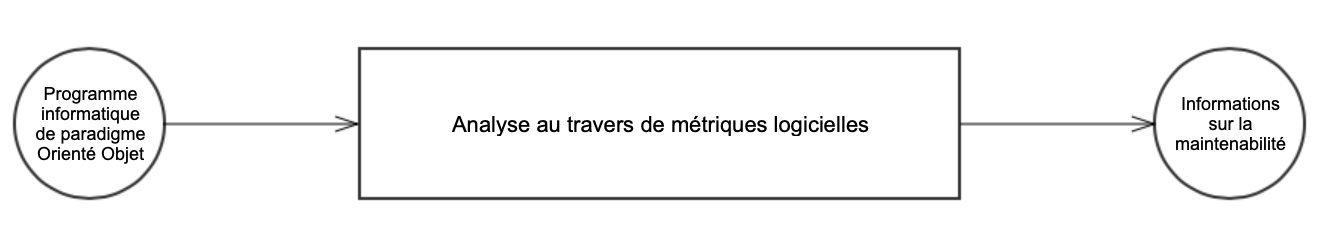
\includegraphics[scale=0.65]{img/intro.png}
    \caption{Vision simplifié du fonctionnement de l'application} 
\end{figure}
    




                    % ------------------------------- %
                    % ----------> DOMAINE <---------- %
                    % ------------------------------- %

\newpage
\section{Description du domaine}

\subsection{Préambule}

Le domaine dans lequel s'inscrit l'application est celui de l'architecture logicielle. En effet, il s'agit ici de déterminer un indicateur du degré de qualité qu'un logiciel possède au regard de la manière dont sont structurés ses composants. Un bon moyen de mesurer une telle chose est d'appliquer le calcul d'une métrique logicielle. Bien que ces métriques soient nombreuses, l'application s'appuiera sur celle définie par Robert Martin\cite{Martin:1994}. Cette section a pour vocation de décrire cette métrique ainsi que tout le vocabulaire nécessaire à sa compréhension.


    

\subsection{Terminologie}
\label{mm:terminologie}

\subsubsection{Dépendances}
    \paragraph{Définition}Une classe (ou ensemble de classes) A \emph{dépend} d'une classe (ou ensemble de classes) B dans le cas où A a besoin de B pour être compilé. Cette \emph{relation de dépendance} peut s'exprimer sous différentes formes :
    \begin{itemize}
        \item \textbf{Dépendance par composition} : A (ou une classe de A) possède un attribut de type B (ou d'une classe de A).
        \item \textbf{Dépendance par application} : A (ou une classe de A) appelle une méthode de B (ou d'une classe de B).
        \item \textbf{Dépendance par héritage / par implémentation} : A (ou une classe de A) est de type B (ou du type d'une classe de B).
        \item \textbf{Dépendance par transitivité} : A dépend de C qui dépend de B.
    \end{itemize}
    
    \paragraph{Couplage} Le degré de couplage est une mesure de l'\emph{interdépendance} entre les différents sous-systèmes d'un programme. On parle de couplage fort pour signifier que l'interdépendance est élevée. On peut étudier cette interdépendance à plusieurs échelles (classes ou ensembles de classes).

    \paragraph{Cohésion}La cohésion représente le degré de liaison et de collaboration des éléments appartenant à un même composant. Une forte cohésion implique que le composant se concentre sur un seul et unique but, une seule et même responsabilité : réaliser des traitements relatifs uniquement à l’intention du composant. A l'inverse, une faible cohésion indique que le composant effectue plusieurs actions sans rapport entre-elles et pourrait certainement être divisé en sous-parties.

\subsubsection{Propriétés d'un design}

    \paragraph{}Afin de comprendre la métrique détaillée dans ce document, il est nécessaire de définir plusieurs propriétés qu'une architecture logicielle peut posséder (ceux-ci sont repris de l'article fondateur de cette métrique, définie par Robert Martin\cite{Martin:1994}) :
    
    \paragraph{Rigidité}Un design rigide est un design qui ne peut être facilement changé. C'est souvent le cas si les composants d'un système sont trop interdépendants. Dans ce cas, un changement dans un composant peut forcer beaucoup d'autres composants à changer également et son impact peut être difficile, si ce n'est impossible, à évaluer.

    \paragraph{Fragilité}Un design fragile est un design qui a tendance à casser à plusieurs endroits si un seul changement est effectué. Dans la plupart des cas, les problèmes engendrés par cette modification surviennent à des endroits sans relation conceptuelle avec la partie ayant subit la modification. De plus, la correction de ces erreurs amène souvent à davantage de nouveaux problèmes. Il devient alors difficile d'estimer la qualité du système.
    
    \paragraph{Robustesse}Un design robuste est l'exact opposé d'un design fragile. En effet, est considéré comme robuste un design au sein duquel un unique changement ne cause pas tout une cascade de problèmes.

    \paragraph{Maintenabilité}Un design maintenable est un design qui peut facilement évoluer. Il faut comprendre par là qu'il doit être facile d'ajouter de nouvelles fonctionnalités ou de modifier le comportement de celles déjà existantes. Un design rigide ou fragile sera peu maintenable.

    \paragraph{Réutilisabilité}Un design réutilisable est un design qui permet la réutilisation de certains de ses composants sans nécessiter d'embarquer ceux dont on ne veut pas. Si ses composants dépendent fortement les uns des autres, le design est dit difficile à réutiliser car il est compliqué d'isoler les composants désirés.
    
\subsubsection{Propriétés d'un composant}
\label{componentProperties}

    \paragraph{}Il s'agit ici de définir plusieurs propriétés que peuvent avoir les composants d'un logiciel. Ces propriétés interviennent dans le calcul de la métrique détaillée plus bas.

    \paragraph{Stabilité}La stabilité désigne la capacité d'un composant à ne pas varier dans le temps. Moins un composant a de risques de changer, plus il est stable. Un composant peut être stable soit parce qu'il n'a aucune dépendance et donc aucune raison de s'adapter à d'autres changements, soit parce que beaucoup d'autres composants dépendent de lui et qu'un changement aurait trop de répercussions sur ceux-ci. Un composant très stable est un composant qui combine les deux propriétés précédentes, à savoir aucune dépendance et beaucoup de composants dépendant de lui.

    \paragraph{Responsabilité}Un composant responsable est un composant dont dépendent de nombreux autres. Un tel composant ne doit pas être souvent modifié car chaque changement peut causer de nombreux problèmes, compte tenu du nombre de composants dépendant de lui. La responsabilité joue en la faveur de la stabilité.
    
    \paragraph{Niveau d'abstraction}L'abstraction, ou le niveau d'abstraction, désigne la proportion d'un composant qui est abstraite (c.à.d. une partie ne comportant que des signatures et pas d'implémentation, dans le but d'être héritée et définie ailleurs). Plus un composant contient de parties abstraites par rapport à sa taille totale, plus il est lui-même abstrait.
    
    \paragraph{Remarque sur les dépendances}Les dépendances d'un composant peuvent être classées en deux types opposés : les bonnes dépendances (Good dependencies) et les mauvaises dépendances (Bad dependencies). Une bonne dépendance est une dépendance dont la cible est très stable. Si A dépend de B et que B est très stable, alors cette dépendance est très bonne. Par opposition, une mauvaise dépendance est une dépendance dont la cible est instable. Ce sont, assez naturellement, ces dépendances qu'il faut éviter.
    

\subsubsection{Catégories de classes ("Class categories")}
    \paragraph{}Dans l'article principal de l'étude\cite{Martin:1994}, R. Martin explique que la métrique qu'il définit a pour but d'étudier les dépendances entres les différentes catégories de classe (\emph{class categories}) d'un programme. Il motive ce choix en précisant que \og \textit{dans une même catégorie, les classes sont censées être très interdépendantes}\fg.
    
    \paragraph{Définition}Afin d'appréhender plus précisément le concept de catégorie de classes utilisé par Robert C. Martin, il est utile de se référer à la définition énoncée par son créateur Grady Booch\cite{Booch:1991}. Booch a mis au point ce concept dans le but de faciliter la mise en oeuvre de représentations structurelles d'applications dans la méthode qui porte son nom. Il définit ce concept de la manière suivante : 
    \begin{quote}
        [A class category is] A logical collection of classes, some of which are visible to other class categories, and others of which are hidden. The classes in a class category collaborate to provide a set of services.
        \begin{flushright}--- G. Booch - \cite{Booch:1991} (p.253)\end{flushright}
    \end{quote}



    \paragraph{Règles d'appartenance à une catégorie}Afin de préciser le concept de catégorie, Martin liste un ensemble de règles (énoncées par ordre d'importance) définissant l'appartenance d'une classe à une catégorie :
    \begin{enumerate}
        \item Les classes appartenant à une même catégorie sont fermées entre elles contre toute force de changement (au sens du principe ouvert/fermé). Cela signifie que si une classe appartenant à une catégorie doit être changée, l'ensemble des classes de cette même catégorie devra changer pour s'adapter. 
        \item Les classes appartenant à une même catégorie ont tendance à être réutilisées ensemble (cette propriété étant une conséquence de leur forte interdépendance).
        \item Les classes appartenant à une même catégorie partagent un but commun.
    \end{enumerate}

    
    
    
    \paragraph{Problématique de cette notion}Il semble complexe de définir un outil qui puisse déterminer de manière autonome l'appartenance d'une classe à une catégorie (au sens de Booch). En effet, la cohésion et l'interdépendance entre les différentes classes d'une catégorie ne décrivent pas forcément la volonté du développeur de créer un ensemble de classes cohérent : cela peut être le reflet d'un code mal structuré (couplage fort).
    
    La détermination de catégorie dans une première analyse de logiciel devrait donc se baser sur la structuration qu'offrent des concepts propres au langage (namespace C++, package Java, etc.).
    

\subsection{Métrique de Martin}
\subsubsection{Présentation et définition}

    \paragraph{}La métrique de Martin a été définie pour la première fois en 1994 par Robert Martin\cite{Martin:1994}. L'auteur l'a par la suite citée au sein d'autres ouvrages\cite{Martin:2003}, et une large bibliographie scientifique mentionne, critique et complète celle-ci\cite{HyryLepp:2009}\cite{BUmetric:2016}\cite{KaurShar:2015}\cite{Spinellis:2006}\cite{Pressman:2000}. La métrique s'articule autour de 2 notions centrales : la stabilité et le niveau d'abstraction (cf. \ref{componentProperties}).

    \paragraph{Définitions}Martin présente une métrique principale : la distance entre une \textit{catégorie} représentée par un point de coordonnées (Instabilité, Abstraction) et la "Main Sequence", une droite représentant le positionnement idéal des catégories. Plus cette distance est grande, moins la classe correspond au pattern recherché. Afin de calculer cette distance, il est nécessaire de calculer plusieurs autres métriques. Voici une liste de celles-ci :
    \begin{itemize}
        \item \textbf{Afferent Coupling, noté Ca} (Le couplage afférent, couplage "entrant") : Il s'agit du nombre de classes externes qui dépendent d'une (ou plusieurs) classes dans la catégorie.
        \item \textbf{Efferent Coupling, noté Ce} (Le couplage efférent, couplage "sortant") : Il s'agit du nombre de classes de la catégorie qui dépendent d'une classe externe.
        \item \textbf{Instability, notée I} (L'instabilité) : Il s'agit d'une quantification de l'instabilité d'une catégorie (cf. \ref{mm:terminologie} pour une définition de la stabilité). Cette métrique fait intervenir les deux précédentes.
        \item \textbf{Abstractness, notée A} (Le niveau d'abstraction) : Il s'agit d'une quantification du niveau d'abstraction d'une catégorie.
        \item \textbf{Distance, notée D (ou Dn pour la version normalisée)} (La distance par rapport à la Séquence Principale, définie ci-dessous.) : Il s'agit d'une mesure de la distance perpendiculaire d'une catégorie à la Séquence Principale. Cette distance donne une idée de la qualité d'une catégorie : le but est de minimiser cette valeur.
    \end{itemize}

\begin{figure}[h!]
    \centering
    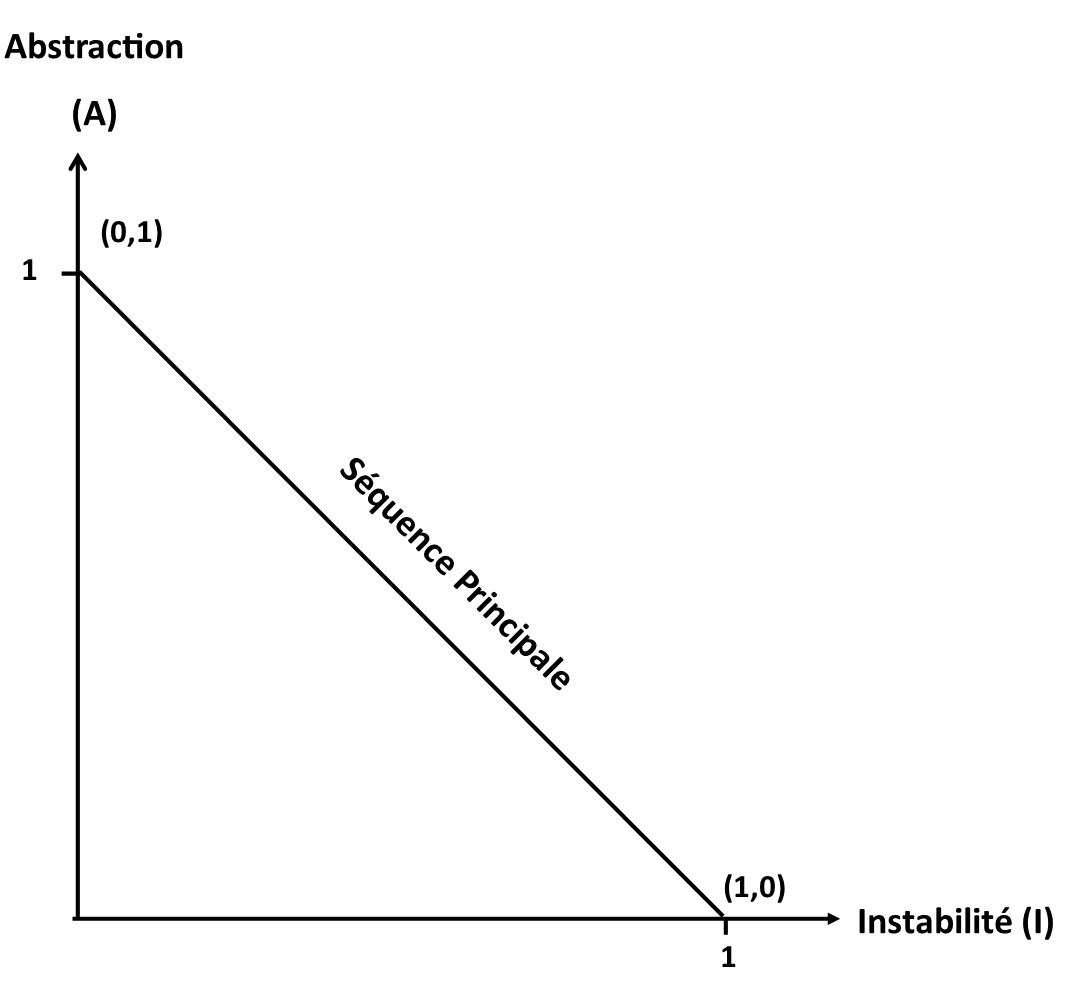
\includegraphics[scale=0.43]{img/MainSequence.png}
    \caption{Séquence principale}
\end{figure}

    \paragraph{}Il est également nécessaire de définir ce qu'est la \textbf{Séquence Principale} ("Main Sequence"). Elle intervient dans le contexte d'une représentation en deux dimensions des métriques. Dans ce plan, une catégorie est représentée par un point dont les coordonnées sont les suivantes : \textbf{(Instabilité, Niveau d'abstraction)}. Les positions idéales se situent en coordonnées (0,1), il s'agit d'une catégorie instable mais entièrement concrète, et (1,0), qui représente une catégorie très stable et entièrement abstraite. Des compromis sont également possibles : il s'agit de la Séquence Principale, une droite passant par (0,1) et (1,0). Les catégories proches de cette droite sont considérées comme bien équilibrées. Dès lors, une faible distance D sera indicatrice de catégorie bien formée alors qu'une distance important indiquera que la catégorie est potentiellement améliorable.
    
\subsubsection{Formalisme}
\label{martin:formalism}

    \paragraph{Variables}Soit \project{} un projet de développement. Un projet \project{} est composé par un ensemble de $n$ ($n > 0$) classes et de $m$ ($m \geq 0$) packages. On note \classUniverse{}, l'univers des classes. \classUniverse{} = $\{\class{}_1, \class{}_2, \dots, \class{}_n\}$ où $c_1, c_2, ... c_n$ représentent les $n$ classes de \project.

    Une catégorie \category{} est un sous-ensemble non-vide de U : \category{} = $ \{\class{}_i, \dots, \class{}_j\} \subseteq$ \classUniverse{}, avec $0 > i, j \geq n$.

    On définit \categoryUniverse{} comme l'ensemble des \category{}. On appelle catégorie élémentaire une catégorie de cardinal 1 (c.à.d. une catégorie composée d'une unique classe).

    \paragraph{Fonctions}On note les fonctions suivantes :
    \begin{itemize}
        \item \dependantClasses{}(\category{}) = Le nombre de classes dépendant d'une catégorie \category{}.
        \item \dependedClasses{}(\category{}, \categoryUniverse{}) = Le nombre de classes dont dépend une catégorie \category{} dans son univers \categoryUniverse{}.
        \item \numberOfMethod{}(\category{}) = Le nombre de méthodes présentes au sein d'une catégorie \category{}.
        \item \numberOfabstractMethod{}(\category{}) = Le nombre de méthodes abstraites présentes au sein d'une catégorie \category{}.
    \end{itemize}

    \paragraph{Calculs}Les différentes métriques définies plus haut sont calculables par application des formules suivantes : 
    \begin{itemize}
        \item Ca(\category{}) = \dependantClasses{}(\category{}) $\in \mathbb{N}$
        
        \item Ce(\category{}, \categoryUniverse{}) = \dependedClasses{}(\category{}, \categoryUniverse{}) $\in \mathbb{N}$
        
        \item A(\category{}) = 
        \numberOfabstractMethod{}(\category{}) /
        {\numberOfMethod{}(\category{})} $\in \lvert 0, 1\rvert$

        \item I(\category{}) = Ce(\category{}) / (Ca(\category{}) + Ce(\category{}) $\in \lvert 0, 1\rvert$
        
        \item \textbf{D(\category{}) = | (A + I - 1) / $\sqrt{2}$ | $\in \lvert 0, 0.707\rvert$}

    \end{itemize}
    
La distance peut se normaliser dans un intervalle de 0 à 1 en utilisant une formule simplifiée :
    \begin{itemize}
        \item Dn(\category{}) = | (A(\category{}) + I(\category{}) - 1) | $\in \lvert 0, 1\rvert$.
    \end{itemize}  

\paragraph{Finalité du calcul} Finalement, on remarque que toutes les métriques participent à calculer la distance à la Séquence Principale. Une fois celle-ci calculée pour toutes les catégories, il est facile de repérer celles auxquelles il semble nécessaire de prêter attention.

\subsection{Intérêts}
    
    \paragraph{Comprendre la métrique}Un intérêt annexe à l'objectif principal de l'application est que son développement est un moyen efficace de comprendre et de mener une réflexion sur la métrique. Ceci permettrait de l'évaluer dans son ensemble et d'apporter des améliorations.
    
    \paragraph{Critique et pistes d'amélioration}
    
    Le problème majeur que l'on peut reprocher à la métrique de Martin est que le résultat du calcul des métriques ne constituent pas des références absolues, ce sont des indicateurs qui peuvent servir à détecter les zones de code auxquelles prêter une attention particulière.
    
    Les métriques décrites par Chidamber et Kemerer\cite{ChidamberKemerer:1994} définissent un  indicateur plus simplifié que les métriques de Martin. En effet, ils définissent six métriques telles que la profondeur de l'arbre d'héritage (DIT), le nombre de fils d'une classe (NOC), le manque de cohésion des méthodes d'une classe (LCOM) et bien d'autres qui sont utiles dans l'étude du couplage et la cohésion au niveau de différentes classes. Certains éléments de ces métriques peuvent servir à améliorer la métrique de Martin.
    
    \begin{quote}
        These metrics should assist software designers in their understanding of the complexity of their design and help direct them to simplifying their work. What the designers should strive for is strong cohesion and loose coupling.
        \begin{flushright}--- C.Kemerer \& S. Chidamber \cite{ChidamberKemerer:1994} (p.229)\end{flushright}
    \end{quote}
    
    \paragraph{}Martin présente sa métrique comme ne s'appliquant qu'aux catégories contenant plusieurs classes. Cependant, en utilisant le formalisme exprimé en section \ref{martin:formalism}, la métrique de Martin peut s'appliquer à l'échelle des classes (catégories élémentaires).
    
    \paragraph{}Telle qu'elle est énoncée, la métrique de Martin considère les dépendances comme toutes égales. Or, une dépendance envers une catégorie stable ne devrait pas avoir le même poids qu'une dépendance envers une catégorie instable. Afin de raffiner le calcul des métriques, une analyse de la globalité de l'arbre des dépendances permettrait d'éliminer les dépendances stables du calcul d'instabilité (ou du moins de minimiser leur poids), en considérant qu'une dépendance stable ne rend pas le composant dépendant instable.
    
\newpage
    
\section{Application au langage Java}

    \paragraph{}L'application aura pour but d'appliquer la métrique à des programmes écrits en langage Java. Dans ce cadre, une clarification de la manière dont certains concepts sont utilisables en Java est nécessaire.

\subsection{Adaptation des notions}

    \paragraph{Catégories de classes}La notion la plus proche de catégorie de classes dans le langage Java est celle de package. Cependant, il existe un glissement sémantique : bien que ce soit souvent le cas en pratique, un package Java n'est pas obligatoirement composé d'un ensemble de classes \emph{collaborant} pour offrir un ensemble de services. Cette notion peut aussi s'appliquer aux modules.

\subsection{Analyse de l'existant}
    \paragraph{}Il existe différents projets qui abordent la question de la maintenabilité de logiciels au travers de l'étude de métriques (on notera que beaucoup d'entre eux exposent les métriques de Chidamber et Kemerer\cite{ChidamberKemerer:1994}). Pour le langage Java, on peut citer JHawk\footnote{\url{http://www.virtualmachinery.com/jhawkprod.htm}} en guise d'exemple. Certains de ces outils s'intègrent à des IDE comme Eclipse ou IntelliJ, ce qui facilite grandement leur mise en place et leur installation.
    
    \paragraph{JDepend}JDepend est un logiciel open source dont le code source est disponible sur la plateforme Github\footnote{\url{https://github.com/clarkware/jdepend}}. Il met en oeuvre la métrique de Martin (et nourrit donc des ambitions similaires à celles de notre application).

    \paragraph{}JDepend procède à une analyse statique des différents fichiers constituant un projet Java. Plus exactement, il analyse les fichiers compilés (\texttt{.class}) composés de bytecode (il peut donc également analyser les archives jar).
    
    \paragraph{}A la suite d'une étude préliminaire du fonctionnement de JDepend, il ressort que celui-ci semble n'extraire que les informations de dépendance entre les packages (principalement au travers des déclarations \textit{import} de Java). Il calcule et fournit alors les dépendances et valeurs de métriques à cette échelle. Il ne peut donc fournir aucune information sur les dépendances entre classes. 
    
    \paragraph{}L'approche de ce projet est différente. En effet, là où JDepend se limite aux packages, notre application adopte une approche \textit{bottom-up} : l'analyse s'effectue au niveau de granularité le plus bas (la classe). A partir des résultats de celle-ci, on peut alors calculer les dépendances et métriques des échelles supérieures sans analyse supplémentaire.
    
    \paragraph{Remarque}Certains travaux se basent sur l'outil JDepend pour analyser des programmes, comme par exemple \textit{Gephi}\footnote{\url{https://dzone.com/articles/visualizing-and-analysing-java}}






                    % ------------------------------- %
                    % ----------> BESOINS <---------- %
                    % ------------------------------- %

\newpage
\section{Expression des besoins}

\subsection{Besoins fonctionnels}

    \paragraph{}Nous n'avons pas réalisé une étude complète\footnote{Une étude préliminaire est exposée en annexe} sur les outils et méthodes d'analyse à utiliser pour l'instant. Les deux choix possibles sont l'analyse de code source ou l'analyse de bytecode. Certains détails techniques n'ont pas encore été fixés et peuvent influencer les différents besoins énoncés ci-dessous.

    \requirement{Evaluer les méthodes d'analyse et définir celle à utiliser}
    {Forte}
    {En amont du développement de l'application, les méthodes d'extraction d'informations concernant les dépendances doivent être évaluées afin de déterminer la plus aisée et rapide à mettre en place. C'est cette solution qui sera retenue pour la suite du projet.}

    \requirement{Générer un ensemble de projets annotés (Création d'une vérité terrain)}
    {Forte}
    {Afin de tester notre implémentation, il sera nécessaire de générer une série de projets Java et de fournir les métriques calculées manuellement.

    Dans ces différents cas d'exemples, seule la structure des dépendances (c.à.d. l'agencement des classes ainsi que les dépendances internes aux méthodes) est importante. Il sera donc inutile d'implémenter des fonctionnalités dans le corps des fonctions.}


\subsubsection{Sélection et structuration de l'entrée}

    \requirement{Sélectionner un projet depuis un répertoire local}
    {Forte}
    {L'utilisateur doit pouvoir renseigner un projet en entrée de l'application depuis le système de fichiers de la machine, sous forme de chemin d'accès au répertoire racine de celui-ci.}
    \testRequirement{S'assurer que l'interface en ligne de commande accepte les chemins corrects (ceux qui mènent vers un répertoire local) et rejette les chemins incorrects (ceux qui mènent vers un répertoire inexistant).}

    \requirement{Lister récursivement le contenu d'un répertoire}
    {Forte}
    {Pour un répertoire donné, l'application doit être en mesure de lister son contenu. Dans le cas d'une analyse du code source (respectivement, d'une analyse du bytecode), l'application devra pouvoir lister l'arborescence des différents fichiers \texttt{.java} (respectivement \texttt{.class}). Si le répertoire donné ne contient pas un projet Java (sous la forme d'un ensemble de \texttt{.class} ou de \texttt{.java}), l'application devra renvoyer une erreur.}

    \requirement{Créer une structure représentative de l'organisation du projet}
    {Forte}
    {L'application devra créer une structure arborescente contenant tous les packages du projet analysé ainsi que les classes qui les composent.}





\subsubsection{Analyse de fichiers}

    \paragraph{}L'application doit être en mesure de réaliser une \textbf{analyse statique} de fichiers. L'analyse de fichiers consistera en la mesure du niveau d'abstraction des classes ainsi que l'extraction des dépendances. Lors de l'analyse, nous ne nous intéresserons qu'à l'ensemble des dépendances sortantes ; nous pourrons déterminer les dépendances entrantes à partir des premières. Cette mesure permettra de déterminer les composantes Ce et A de la métrique.

    \paragraph{}Les différentes dépendances que l'application devra extraire sont les suivantes, par ordre de priorité d'implémentation (les quatre premières sont d'importance égales et leur implémentation est de priorité très haute) :
    \begin{itemize}
        \item Dépendances par héritage/implémentation
        \item Dépendances par agrégation/composition
        \item Dépendances de signature (paramètres ou type de retour d'une méthode)
        \item Dépendances internes au corps d'une méthode
        \item Dépendances liées à la généricité (héritage d'un paramètre générique)
    \end{itemize}

    \paragraph{}On considérera les classes internes comme faisant partie intégrante de leur classe englobante.

    \requirement{Extraire les dépendances par héritage/implémentation}
    {Forte}
    {L'application devra extraire les dépendances de type héritage/implémentation. Cette information se trouve dans la déclaration de la classe.}

    \requirement{Extraire les dépendances par agrégation/composition}
    {Forte}
    {L'application devra extraire les dépendances de type agrégation/composition. Cette information se trouve dans la liste des attributs de la classe. Cela implique que l'application devra être en mesure de lister les attributs d'une classe et leurs types.}

    \requirement{Extraire les dépendances de signature}
    {Forte}
    {L'application devra extraire les dépendances de signature. Cette information se trouve dans la signature des méthodes. Il s'agit des paramètres ou du type de retour de celles-ci.}

    \requirement{Extraire les dépendances internes au corps d'une méthode}
    {Moyenne}
    {L'application devra extraire les dépendances internes au corps d'une méthode. Il s'agit de l'instanciation d'un objet ou d'un appel de méthode statique.}

    \requirement{Extraire les dépendances liées à la généricité}
    {Faible}
    {L'application devra extraire les dépendances dues à la généricité. Cette information peut se trouver dans la déclaration de la classe, dans la signature ou dans le corps des méthodes. Cette dépendance est plus compliquée à mettre en place car elle peut prendre plusieurs formes.}
    
    \requirement{Mesurer le nombre de méthodes d'une classe}
    {Forte}
    {Afin d'implémenter la fonction \numberOfMethod{}, il faudra mettre en place une méthode permettant de compter le nombre de méthodes qu'une classe définit.}
    
    \requirement{Mesurer le nombre de méthodes abstraites d'une classe}
    {Forte}
    {Afin d'implémenter la fonction \numberOfabstractMethod{}, il faudra mettre en place une méthode permettant de compter le nombre de méthodes abstraites qu'une classe définit.}


\subsubsection{Exploitation de la métrique}

    \requirement{Calculer le couplage afférent (Ca)}
    {Forte}
    {A partir du couplage efférent (Ce) de toutes les classes, l'application devra déterminer le couplage afférent (Ca) de chaque classe en examinant le nombre de classes ayant des dépendances sortantes vers cette classe.}

    \requirement{Calculer la composante d'instabilité de la métrique}
    {Forte}
    {L'application devra être en mesure d'effectuer le calcul de la composante I de la métrique pour une classe donnée (catégorie élémentaire) à partir de la formule définie par Martin : I(\category{}) = Ce(\category{}) / (Ca(\category{}) + Ce(\category{}).}

    \requirement{Calculer la composante de distance de la métrique}
    {Forte}
    {L'application devra être en mesure d'effectuer le calcul de la composante Dn de la métrique pour une classe (catégorie élémentaire) donnée à partir de la formule définie par Martin : Dn(\category{}) = |(A(\category{}) + I(\category{}) - 1)|.}    

    \requirement{Générer un graphe de dépendances}
    {Forte}
    {A partir des dépendances extraites de l'analyse de fichiers, l'application devra être en mesure de générer une structure de données représentative de l'interdépendance entre les différentes classes du projet : un graphe de dépendances. 
    
    Le graphe de dépendances est défini comme un graphe orienté composé d'un ensemble de $n$ noeuds représentant les $n$ classes de l'analyse et d'un ensemble de $p$ arcs représentant les dépendances entre celles-ci. Étant donné que l'application fait la différence entre chaque type de dépendance, il peut y avoir plusieurs arcs d'un noeud vers un autre (un par type de dépendance).
    
    A partir de ce graphe de dépendances de classes, il est possible de passer à un niveau d'échelle supérieur en fusionnant les noeuds pour les regrouper par catégorie (package par exemple) et en ne conservant que les arcs sortants et entrants dans ces super-noeuds.}

    \requirement{Générer des tableaux exposant les composantes de la métrique}
    {Forte}
    {L'application devra être en mesure de créer des tableaux exposant les différentes composantes de la métrique, celles récupérées au travers de l'analyse de fichiers (Ce et A) et celles calculées par la suite (Ca, I et D). On pourra obtenir les informations relatives au changement d'échelle à partir des données du graphe de dépendances.}


\subsubsection{Réalisation de rapport d'analyse}

    \paragraph{}L'application devra permettre de générer des fichiers exposant les différentes métriques qu'elle aura traité. Ces fichiers pourront ensuite être interprétés par des outils externes.

    \requirement{Générer des fichiers DOT exposant le graphe des dépendances}
    {Forte}
    {L'application devra être en mesure de générer des fichiers au format DOT. Ces fichiers contiendront les graphes de dépendance calculés précédemment. Il y aura un fichier par échelle d'analyse (catégories). Les noeuds contiendront le nom des catégories (nom de classe, de package,...) associé à leur valeur d'instabilité. Ces fichiers pourront ensuite être interprétés par des outils tels que GraphViz.}
    
    \requirement{Générer des fichiers CSV exposant les métriques}
    {Forte}
    {L'application devra être en mesure de générer des fichiers au format CSV. Ils contiendront les valeurs des différentes composantes de la métrique. Tout comme les fichiers DOT, il en existera un par échelle d'analyse. Ces fichiers pourront ensuite être interprétés par des outils tels que Libre Office Calc.}


\subsection{Besoins non fonctionnels}

    \requirement{Documentation}
    {Forte}
    {La documentation de l'application sera scindée en deux documents : l'architecture générale et le manuel d'utilisation. Ceux-ci seront produits dans le format \LaTeX{} afin de permettre leur intégration dans le rapport terminal de l'UE.
    
    \textbf{Architecture générale} : Pour aider les développeurs à modifier / adapter / ajouter des fonctionnalités à l'application.
    
    \textbf{Manuel d'utilisation} : Pour aider l'utilisateur à prendre en main l'application.}


    \requirement{Portabilité}
    {Moyenne}
    {L'application devra limiter son assujettissement à des outils externes, particulièrement si ceux-ci sont non portables. Des exceptions à cette règle sont envisageable si un outil s'avère pouvoir apporter un avantage important à l'application.}

    \requirement{Modularité}
    {Forte}
    {Les algorithmes de calcul des métriques doivent pouvoir être aisément modifiés. L'application doit adopter une architecture lui permettant de s'adapter sans nécessiter de changements conséquents.}

    \requirement{Configuration}
    {Faible}
    {La possibilité de modifier certains paramètres de l'application (par exemple, il pourrait être possible de paramétrer une pondération à appliquer à chaque type de dépendance dans le calcul de la métrique) à l'aide d'un fichier de configuration peut être implémentée en guise d'alternative à la modification directe d'un composant dans le code. La présence d'une telle fonctionnalité est optionnelle.}

% ----------> BIBLIOGRAPHY
\pagebreak
\bibliographystyle{unsrt}
\bibliography{references}






\newpage
\section{Annexes}

\subsection{Étude préliminaire sur l'évaluation de la méthode d'analyse}

\begin{table}[h!]
    \centering
    \caption{Tableau comparatifs des méthodes d'analyse}
    \begin{tabular}{|c|c|c|}
        \hline
        \textbf{Méthodes} & \textbf{Code source} & \textbf{Bytecode} \\
        \hline
        Outils        &  \makecell{Bison et Flex}         & \makecell{ASM,\\ Outils d'introspection du JDK}                 \\
        \hline
        Avantages     &  \makecell{Pas de compilation}                      &  \makecell{Plus d'outils disponibles}                   \\
        \hline
        Inconvénients & \makecell{Moins d'outils existants}            &  \makecell{Nécessite de compiler}                   \\
        \hline
    \end{tabular}
\end{table}


\subsection{Exemple de projet annoté}
    \paragraph{}Dans le but de vérifier que l'application calcule les valeurs de métrique correctement, il est nécessaire d'écrire de petits logiciels simples présentant des configurations de dépendances différentes. Nous donnons ici un exemple élémentaire de projet annoté.

\begin{minipage}{7.5cm}
\begin{lstlisting}[caption=Classe Vehicle]
public abstract class Vehicle {
    private int nbWheel;
    private ArrayList<Wheel> wheels;
    public abstract void move();
    public void setNbWheel(int i) { }
    public void addWheel(Wheel w) { }
}
\end{lstlisting}
\end{minipage}
\hspace{0.5cm}
\begin{minipage}{6cm}
\begin{lstlisting}[caption=Enumeration Material]
public enum Material {
    Plastic,
    Metal,
    Carbon
}
\end{lstlisting}
\end{minipage}
\vspace{0.5cm}
\begin{lstlisting}[caption=Classe Airplane]
public class Airplane extends Vehicle {
    @Override
    public void move() { /* ... */ }
}
\end{lstlisting}
\begin{lstlisting}[caption=Classe Car]
public class Car extends Vehicle {
    @Override
    public void move() { /* ... */ }
}
\end{lstlisting}
\begin{lstlisting}[caption=Classe Wheel]
public class Wheel {
    private Material material;
    public Material getMaterial() { return this.material; }
    public void setMaterial(Material m) { this.material = m; }
}
\end{lstlisting}



\begin{figure}
    \centering
    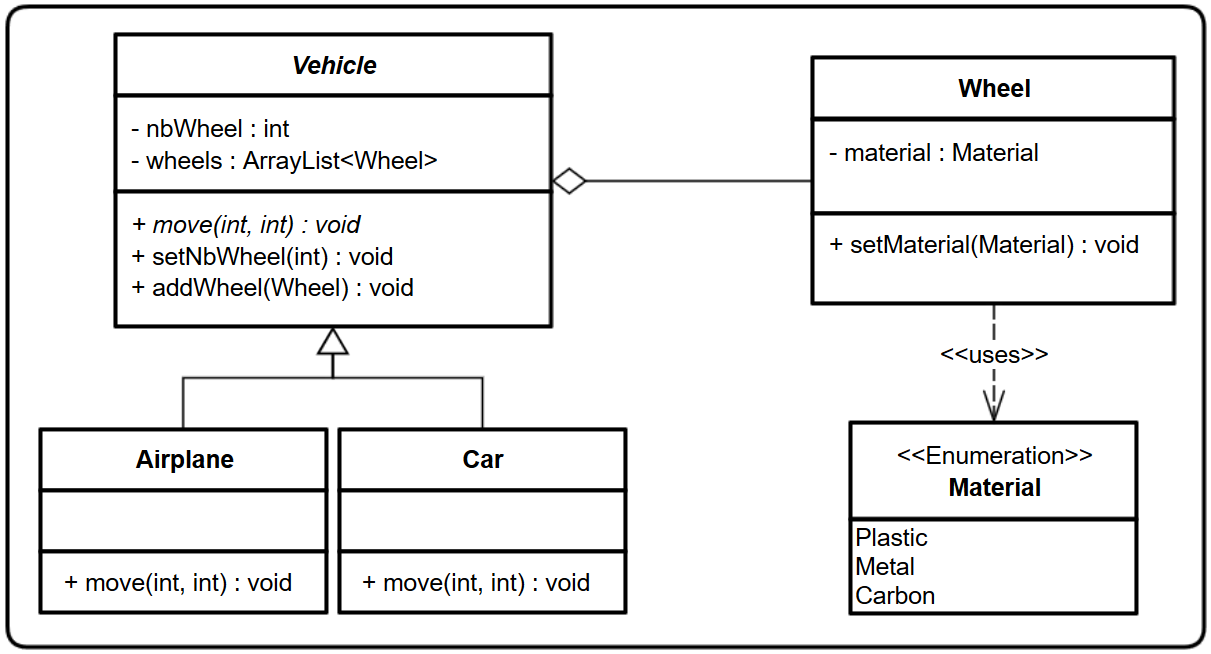
\includegraphics[scale=0.5]{img/uml_example.png}
    \caption{Diagramme de classe du projet exemple}
\end{figure}


\begin{table}[H]\caption{Tableau exposant les métriques}
    \centering
    \begin{tabular}{|c|c|c|c|c|c|}
        \hline
        \textbf{Catégorie} & \textbf{Ca} & \textbf{Ce} & \textbf{A} & \textbf{I} & \textbf{Dn} \\
        \hline
        \textbf{Vehicle} & 2 & 1 & 0.33 & 0.33 & 0.33 \\
        \hline
        \textbf{Material} & 1 & 0 & 0 & 0 & 1 \\
        \hline
        \textbf{Airplane} & 0 & 1 & 0 & 1 & 0  \\
        \hline
        \textbf{Car} & 0 & 1 & 0 & 1 & 0 \\
        \hline
        \textbf{Wheel} & 1 & 1 & 0 & 0.5 & 0.5 \\
        \hline
    \end{tabular}
\end{table}


\begin{figure}
    \centering
    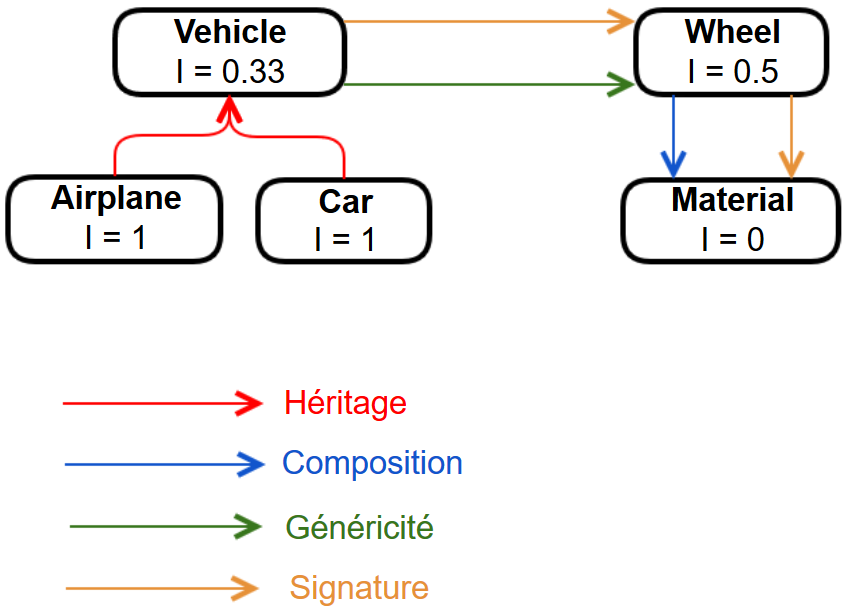
\includegraphics[scale=0.5]{img/gdd_example.png}
    \caption{Graphe des dépendances du projet exemple}
\end{figure}



\subsection{Diagramme de Gantt}
    \begin{sidewaysfigure}[htbp]
        \centering
        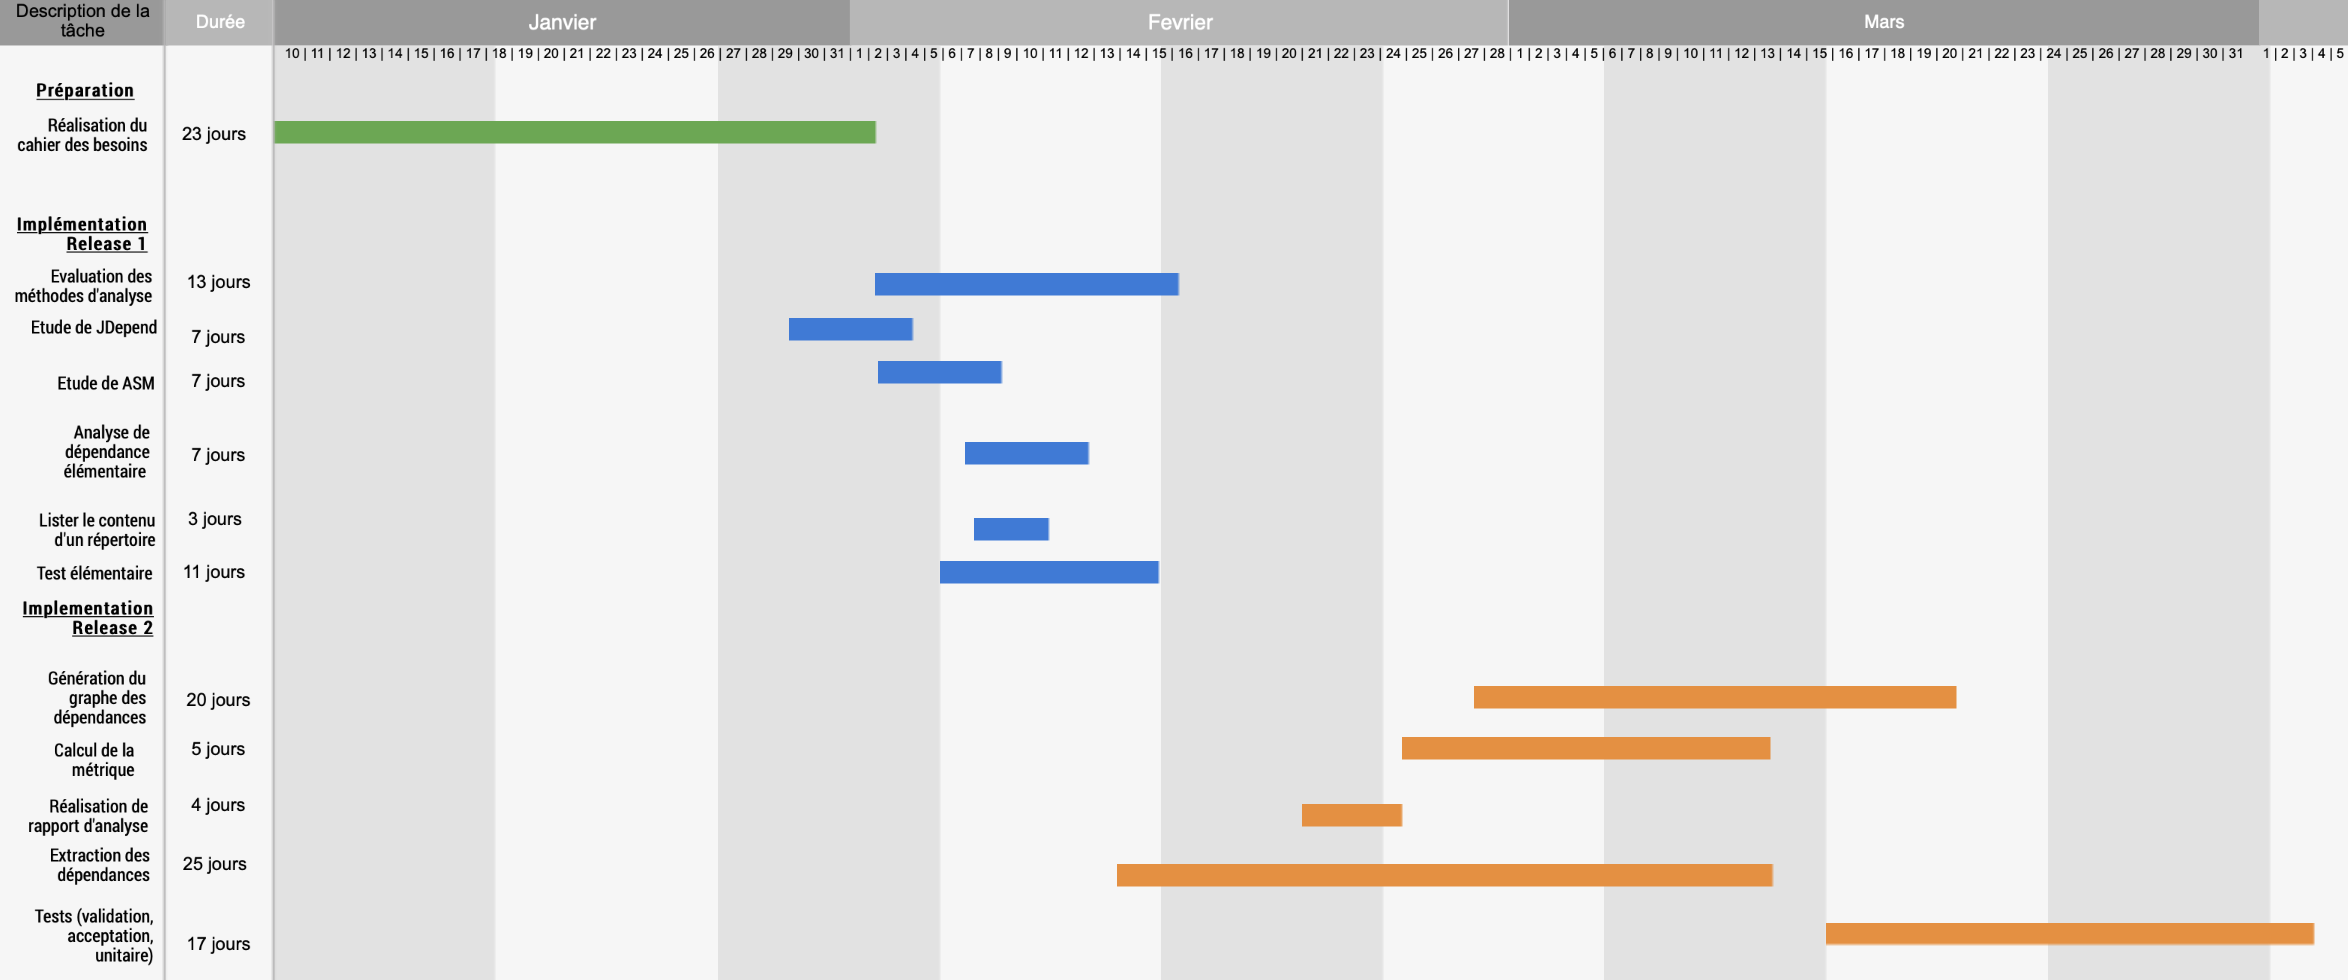
\includegraphics[width=\linewidth, height=\textheight,keepaspectratio]{img/Gantt.png}
    \end{sidewaysfigure}
    
    
    

\end{document}
